\documentclass[12pt,a4paper]{article}
\usepackage{amsmath,amssymb,amsthm}
\usepackage{graphicx}
\usepackage[margin=1in]{geometry}
\usepackage{enumitem}
\usepackage{hyperref}
\usepackage{url}
\usepackage{tikz}
\usepackage{tikz-cd}
\usepackage{tikz-3dplot}
\usetikzlibrary{angles,quotes,arrows.meta,calc,babel,3d,positioning}
\usepackage{lipsum}
\usepackage{listings}
\usepackage{fancyhdr}
\usepackage{xcolor} % Added for colors
\usepackage{titlesec} % Added for title formatting
\usepackage{array}
\usepackage{booktabs}
\usepackage{float}
\usepackage{wrapfig} % For text wrapping around figures
\usepackage{microtype}

% Better figure placement defaults
\setcounter{topnumber}{2}
\setcounter{bottomnumber}{2}
\setcounter{totalnumber}{4}
\renewcommand{\topfraction}{0.85}
\renewcommand{\bottomfraction}{0.85}
\renewcommand{\textfraction}{0.15}
\renewcommand{\floatpagefraction}{0.7}

% Define colors
\definecolor{titlecolor}{RGB}{0, 51, 102}

% Fix headheight warning
\setlength{\headheight}{14.5pt}
\addtolength{\topmargin}{-2.5pt}

% Consistent theorem/proof environments
\newtheorem{theorem}{Theorem}
\newtheorem{lemma}[theorem]{Lemma}
\newtheorem{corollary}[theorem]{Corollary}
\theoremstyle{definition}
\newtheorem{definition}[theorem]{Definition}
\newtheorem{problem}{Problem}

% Set up headers
\pagestyle{fancy}
\fancyhf{} % Clear all header and footer fields
\fancyhead[L]{Victor Gurbani}
\fancyhead[R]{JuFo 2026}
\fancyfoot[C]{\thepage} % Page number in center of footer

% Define a separate first page style with no numbers
\fancypagestyle{firstpage}{
    \fancyhf{} % Clear all header and footer fields
    \renewcommand{\headrulewidth}{0pt} % Remove header rule
    \renewcommand{\footrulewidth}{0pt} % Remove footer rule
}

% Create a custom title command
\renewcommand{\maketitle}{
    \begin{titlepage}
        \centering
        \vspace*{1cm}
        {\color{titlecolor}\rule{\linewidth}{1pt}}
        \vspace{1.5cm}

        {\fontsize{28}{34}\selectfont\color{titlecolor}\textbf{Empirische Musikalische Kartographie} \par Eine quantitative Analyse der stilistischen Evolution von Bach bis Debussy\par}

        \vspace{1.5cm}
        {\color{titlecolor}\rule{\linewidth}{1pt}}
        \vspace{2cm}
        
        {\Large\textbf{Victor Gurbani}\par}
        \vspace{0.5cm}
        {\large\today\par}
        
        \vfill
        % Optional: Add a simple decorative element
        % \begin{tikzpicture}[remember picture, overlay]
        %     \draw[color=titlecolor, line width=0.5pt] 
        %         ($(current page.center) + (-3,0)$) -- ($(current page.center) + (3,0)$);
        % \end{tikzpicture}
    \end{titlepage}
}

\begin{document}

\maketitle
\setcounter{page}{1}
\pagenumbering{arabic}
\newpage

    \tableofcontents

\newpage

\section{Fachliche Kurzfassung}
Die stilistische Evolution von der kontrapunktischen Strenge des Barock bis zur klanglichen Farbigkeit des Impressionismus ist musikwissenschaftlich umfassend beschrieben, ihre empirische Quantifizierung stellt jedoch eine methodische Herausforderung dar. Dieses Projekt entwickelt eine \emph{Empirische Musikalische Kartographie}, die diese Lücke durch Integration moderner computergestützter Verfahren mit interpretierbarer Merkmalsextraktion schließt.

Die Methodik basiert auf drei komplementären Säulen: (1)~Kuratierung eines lizenzsicheren, balancierten Klavierkorpus mit 144 Partituren (je 36 von Johann Sebastian Bach, Wolfgang Amadeus Mozart, Frédéric Chopin und Claude Debussy) aus dem 254\,077 Partituren umfassenden PDMX-Archiv, (2)~Entwicklung einer Python-Pipeline zur Extraktion von 36 interpretierbaren harmonischen, melodischen und rhythmischen Merkmalen mittels \texttt{music21},\footnote{Die Zahl 36 für Werke/Komponist und die Zahl 36 für Merkmale sind unabhängig; die Übereinstimmung ist zufällig.} (3)~statistische Kartierung durch ANOVA, Tukey-HSD-Tests und Principal Component Analysis (PCA) mit Korrektur für multiples Testen (Bonferroni und Benjamini--Hochberg FDR).

Die Analyse identifiziert 29 statistisch robuste Metriken (FDR $q<0{,}05$), die stilistische Unterschiede quantifizieren. Chromatische Dichte (\texttt{pitch\_class\_entropy}), Dissonanzraten (\texttt{dissonance\_ratio}) und rhythmische Entropie trennen insbesondere Debussy deutlich von Mozart; Chopin liegt im Merkmalsraum häufig zwischen den Gruppen.

Die Signale sind dabei nicht nur qualitativ, sondern auch statistisch extrem stark: exemplarisch ergeben sich in der Einweg-ANOVA etwa für \texttt{pitch\_range\_semitones} $p<1{,}8\times 10^{-19}$ und für \texttt{dissonance\_ratio} $p<2{,}7\times 10^{-15}$; auch rhythmische Marker wie \texttt{std\_note\_duration} ($p\approx1{,}5\times10^{-10}$) und \texttt{rhythmic\_pattern\_entropy} ($p\approx5{,}0\times10^{-10}$) bleiben nach FDR-Korrektur robust.

Die PCA-Projektion visualisiert diese Differenzierung als dreidimensionale Landkarte: Bach und Mozart liegen gemeinsam in der Common-Practice-Region (ähnliche PC1-Werte), werden jedoch entlang PC2 (Dichte/Klarheit) getrennt. Debussy erscheint als isolierte impressionistische Insel, Chopin positioniert sich als Brückenfigur zwischen den Epochen. Diese quantitative Verortung bestätigt empirisch die musikhistorische These von Chopins Scharnierfunktion: Er bewahrt klassische kadenzielle Strukturen, während er harmonisch-melodisch in Richtung Impressionismus innoviert.

Alle Skripte, Daten und Visualisierungen sind dokumentiert und ermöglichen reproduzierbare Folgeuntersuchungen zur stilistischen Evolution in der westlichen Kunstmusik.

\section{Motivation und Fragestellung}
Ein musikalisch ungeschulter Zuhörer erkennt intuitiv den stilistischen Kontrast zwischen einer Fuge von Johann Sebastian Bach und einem Prélude von Claude Debussy. Bach repräsentiert kontrapunktische Präzision, klare metrische Strukturen und diatonische Harmonik; Debussy nutzt parallele Akkorde, pentatonische und ganztonale Skalen sowie polyrhythmische Schichtungen zur Erzeugung von Klangfarben. Zwischen diesen Polen liegt ein reiches Spektrum stilistischer Ausdrucksformen, das durch Wolfgang Amadeus Mozart (Klassik) und Frédéric Chopin (Romantik) repräsentiert wird.

Ziel dieser Arbeit ist es, diese intuitive Unterscheidung so zu formalisieren, dass ein Algorithmus den Stilunterschied zwischen der Common-Practice-Periode (Bach/Mozart) und der späten Romantik bzw. dem Impressionismus (Chopin/Debussy) anhand transparenter, interpretierbarer Merkmale ``hören'' kann -- ohne Black-Box-Modell und ohne manuelle Annotation von Einzelereignissen.

Während die musikwissenschaftliche Literatur diese Evolution qualitativ umfassend beschreibt, fehlt es an empirischen, interpretierbaren Quantifizierungen. Frühere computergestützte Ansätze litten unter zwei komplementären Schwächen: Vereinfachte Metriken (z.\,B.\ reine Notenstatistik) erlaubten nur oberflächliche Aussagen, während komplexe Black-Box-Modelle (neuronale Netze) zwar trennscharf, aber musikologisch intransparent waren.\footnote{Vgl.\ \cite{Simonetta2025} für eine systematische Übersicht über Composer-Identification-Ansätze.}

Lin-Jengs Pionierarbeit von 1987\footnote{\cite{LinJeng1987}.} versuchte bereits, Mozart, Chopin und Debussy mittels Prolog-Regeln zu unterscheiden, war jedoch durch manuelles DARMS-Encoding, kleine Stichproben und begrenzte Rechenkapazität limitiert. Moderne Ressourcen -- das 2024 veröffentlichte PDMX-MusikXML-Archiv\footnote{\cite{PDMX2024}.} mit 254\,077 Partituren und die etablierte \texttt{music21}-Bibliothek\footnote{\cite{Cuthbert2010}.} -- ermöglichen nun eine skalierbare, transparente Neubearbeitung dieser Fragestellung.

\subsection{Forschungsfragen}
Die zentrale Forschungsfrage dieses Projekts lautet:

\begin{quote}
    \textbf{Primärfrage:} Inwieweit kann ein kuratierter Satz interpretierbarer Merkmale in Verbindung mit robuster statistischer Analyse eine empirische Landkarte erstellen, die die stilistische Trennung und Evolution zwischen Bach, Mozart, Chopin und Debussy quantifiziert?
\end{quote}

Daraus leiten sich zwei spezifische Teilfragen ab:

\begin{enumerate}
    \item \textbf{Merkmals-Identifikation:} Welche interpretierbaren Merkmale (z.\,B.\ Dissonanzrate, rhythmische Entropie, chromatische Dichte) erweisen sich als stärkste statistisch signifikante Indikatoren zur Unterscheidung der vier Komponisten?
    
    \item \textbf{Narrative Validierung:} Bestätigt, widerlegt oder nuanciert die quantitative Landkarte etablierte musikwissenschaftliche Narrative -- insbesondere Chopins oft postulierte, aber selten quantifizierte Rolle als Brückenfigur zwischen klassischer Klarheit und impressionistischer Innovation?
\end{enumerate}

Die Beantwortung dieser Fragen erfordert die Integration von Korpuslinguistik, Signalverarbeitung und multivariater Statistik -- eine methodische Herausforderung, die dieses Projekt systematisch adressiert.

\section{Hintergrund und theoretische Grundlagen}
\subsection{Musikwissenschaftlicher Kontext}
Die Auswahl der vier Komponisten deckt zentrale Epochen der westlichen Musikgeschichte ab:\footnote{Vgl. etwa \cite{DebussyCharacteristics,ChopinTransformations}.}
\begin{itemize}
    \item \textbf{Johann Sebastian Bach (Barock)}: polyphone Dichte, kontrapunktische Strenge, funktionale Harmonik.
    \item \textbf{Wolfgang Amadeus Mozart (Klassik)}: homophone Klarheit, symmetrische Phrasen, kadenzielle Disziplin.
    \item \textbf{Frédéric Chopin (Romantik)}: essentielle Chromatik, rubatohafte Rhythmen, expressive Texturen.
    \item \textbf{Claude Debussy (Impressionismus)}: planierende Akkorde, modale und ganztonale Skalen, polyrhythmische Schichtungen.
\end{itemize}

\subsection{Computational-Musicology-Kontext}
Frühe Versuche, diese Komponisten algorithmisch zu unterscheiden, wie Lin-Jengs Arbeit von 1987,\footnote{\cite{LinJeng1987}.} litten unter kleinem Korpus, manuellem Encoding und begrenzten Werkzeugen. Aktuelle Übersichtsarbeiten kritisieren die Dominanz schwer interpretierbarer Modelle oder ungenügender Validierung.\footnote{\cite{Simonetta2025}.} Dieses Projekt nutzt moderne Ressourcen: das 2024 veröffentlichte PDMX-MusikXML-Archiv\footnote{\cite{PDMX2024}.} und die \texttt{music21}-Bibliothek\footnote{\cite{Cuthbert2010}.}, um eine skalierbare, transparent dokumentierte Analyse umzusetzen. Tabelle~\ref{tab:evolution} vergleicht den methodischen Fortschritt.

\begin{table}[H]
    \centering
    \caption{Evolution der Methodik im stilistischen Vergleich}\label{tab:evolution}
    \begin{tabular}{p{3.2cm}p{5cm}p{6cm}}
                \toprule
        \textbf{Aspekt} & \textbf{Lin-Jeng (1987)} & \textbf{Diese Arbeit (2026)} \\
        \midrule
        Korpus & Manuell kodierte Teilmenge & 144 auto-kuratierte Solo-Klavierwerke aus $>$250\,000 Partituren \\
        Datenformat & DARMS & MusicXML / \texttt{music21}-Objekte \\
        Analyse & Prolog-Regeln, Mustererkennung & Python-Pipeline mit 36 Merkmalen, CLI-Tools \\
        Zielsetzung & Klassifikation & Statistische Kartographie (ANOVA \& PCA) \\
        \bottomrule
    \end{tabular}
\end{table}

\section{Vorgehensweise, Materialien und Methoden}
Die Pipeline wurde vollständig in Python~3.10 entwickelt (\texttt{pandas}, \texttt{numpy}, \texttt{scipy}, \texttt{scikit-learn}, \texttt{plotly}, \texttt{music21}). Alle Skripte liegen im Verzeichnis \texttt{src/}.

\subsection{Materialien: Kuratierung des PDMX-Korpus}
\begin{itemize}
    \item \textbf{Rohmaterial}: PDMX-CSV (Metadaten), zugehörige MusicXML-Dateien, JSON-Metadaten (Instrumente, Instrumentationstexte).
    \item \textbf{Problem}: heterogene Schreibweisen, Arrangements, Ensembles, Mehrfachfassungen.
    \item \textbf{Lösung}: \texttt{src/corpus\_curation.py} filtert in mehreren Stufen:
    \begin{enumerate}
        \item Normalisierung der Komponistennamen mit \texttt{ComposerRule} (Token-Listen gegen Aliasformen, Ausschluss von Familienmitgliedern).
        \item Lizenz- und Qualitätsfilter (\texttt{subset:rated\_deduplicated}, \texttt{subset:no\_license\_conflict}, \texttt{is\_best\_unique\_arrangement}).
        \item Instrumentationskontrolle über JSON-Felder, Freitext und \texttt{music21}-Instrumente, um reine Solo-Klavierwerke zu sichern.
        \item Balancierung: Clipping auf die kleinste Anzahl gültiger Werke pro Komponist (36) verhindert Verzerrungen.
    
    \end{enumerate}
    \item \textbf{Ergebnis}: 144 Partituren, Ø 148{,}2 Takte, Ø 2,1 Stimmen, 71\,585 Viertelnoten (\textasciitilde13,3 Stunden bei 90 BPM).
\end{itemize}

Zwischendiagnostik (\texttt{--skip-}\,Flags, unterschiedliche Rating-Schwellen) wurde automatisiert protokolliert und zeigte, dass Lockerungen zwar die Stückzahl erhöhen, aber Lizenzrisiken und starke composer bias erzeugen.

\subsection{Methode: Die Drei-Säulen-Feature-Pipeline}
Für jede Partitur werden harmonische, melodische und rhythmische Deskriptoren erzeugt:\footnote{Details siehe \texttt{ShortArticle.md} und \texttt{Article.md}.}
\begin{description}
    \item[Harmonik (16 Merkmale)] \texttt{music21.stream.Score.chordify()} erstellt einen Akkordstream; es folgen Berechnung von Akkordqualitätsanteilen, harmonischer Dichte, Modal-Interchange-Raten sowie Klassifikation nichtakkordischer Töne (Durchgänge, Vorhalte, Appoggiaturen). Roman-Numeral-Analysen liefern Kadenzenstatistiken.
    \item[Melodik (11 Merkmale)] Stimmen werden expandiert, um Ambitus (\texttt{pitch\_range\_semitones}) und Tonklassenstatistiken zu erfassen. Intervall-basierte Melodik wird aus dem oberen System (erstes \texttt{Part} in MusicXML; Proxy für die rechte Hand/Sopranlage) abgeleitet, um Polyphonie nicht vollständig zu ``flatten''. Für Stimmführungsmetriken wird pro Zeitpunkt die höchste Note im oberen System mit der tiefsten Note im unteren System verglichen; daraus ergeben sich Anteile an Gegen-, Parallel- und Oblique-Motion.
    \item[Rhythmik (9 Merkmale)] Gleitfenster analysieren Dauerverteilungen, Downbeat-Betonung, Synkopationen, mikro-rhythmische Dichte und Cross-Rhythm-Mismatches zwischen Händen.
\end{description}

Tabelle~\ref{tab:features} erklärt zentrale Merkmale, die später als signifikant identifiziert wurden.

\begin{table}[H]
    \centering
    \caption{Ausgewählte interpretierbare Merkmale}\label{tab:features}
    \begin{tabular}{p{3.5cm}p{2.5cm}p{7.5cm}}
                \toprule
        \textbf{Merkmal} & \textbf{Säule} & \textbf{Beschreibung} \\
        \midrule
        \texttt{pitch\_range\_semitones} & Melodik & Tonumfang zwischen tiefster und höchster Note eines Stücks (Halbtonschritte). \\
        \texttt{dissonance\_ratio} & Harmonik & Anteil dissonanter Akkord-Events im \texttt{chordify()}-Stream (\texttt{Chord.isConsonant()==False}). \\
        \texttt{pitch\_class\_entropy} & Melodik & Shannon-Entropie der verwendeten Tonklassen, Indikator für Chromatik. \\
        \texttt{rhythmic\_pattern\_entropy} & Rhythmik & Entropie eines Sliding-Window-Rhythmus-Profils, misst rhythmische Vielfalt. \\
        \texttt{std\_note\_duration} & Rhythmik & Standardabweichung der Notenlängen; höher bedeutet Mischung aus sehr kurzen und sehr langen Noten (Proxy für rubatohafte Fluidität). \\
        \texttt{syncopation\_ratio} & Rhythmik & Synkopationsanteil (Offbeat-Ereignisse relativ zu metrisch starken Positionen). \\
        \texttt{downbeat\_emphasis\_ratio} & Rhythmik & Anteil der Ereignisse auf Downbeats, misst metrische Klarheit. \\
        \bottomrule
    \end{tabular}
\end{table}

\subsection{Statistische Analysemethode}
\begin{enumerate}
    \item \textbf{ANOVA}: Einweg-ANOVA pro Merkmal testet globale Mittelwertunterschiede zwischen vier Gruppen. Die 36 Tests wurden auf Mindeststichproben (36 Werke/Komponist) geprüft.
    \item \textbf{Tukey HSD}: Bei signifikanten ANOVA-Ergebnissen identifiziert Tukey HSD die betroffenen Komponistenpaare mit Konfidenzintervallen und adjustierten \textit{p}-Werten.
    \item \textbf{Multiple-Testing-Korrektur}: Bonferroni ist bei 36 Tests streng (14 statt 29 Treffer bei \(\alpha=0{,}05\)). Benjamini--Hochberg FDR (\(q<0{,}05\)) bestätigt in der aktuellen Auswertung ebenfalls 29 Merkmale; im Export werden dennoch FDR-adjustierte \textit{p}-Werte berichtet.\footnote{Vgl.\ \cite{Benjamini1995}.}
    \item \textbf{PCA}: Für die PCA wurden aus den 36 Merkmalen reine Zähl- und Größenmerkmale entfernt (\texttt{note\_count}, \texttt{note\_event\_count}, \texttt{chord\_event\_count}, \texttt{chord\_quality\_total}, \texttt{roman\_chord\_count}, \texttt{dissonant\_note\_count}), sodass eine standardisierte 144×30-Matrix entsteht. Die PCA wurde mit Seed 42 durchgeführt; PC1--PC3 erklären 48{,}2\% der Varianz (22{,}3\%, 16{,}1\%, 9{,}8\%). Gaußsche Dichtewolken (Plotly-Isosurfaces) visualisieren Cluster.
\end{enumerate}

\subsection{Software-Architektur und Reproduzierbarkeit}
Die gesamte Analysepipeline wurde als modulares CLI-System implementiert, das vollständige Reproduzierbarkeit gewährleistet:

\begin{itemize}
    \item \textbf{Korpus-Kuratierung} (\texttt{corpus\_curation.py}): Filtert PDMX-Metadaten nach Komponist, Lizenz, Besetzung und Qualität; balanciert auf kleinste Gruppengröße.
    \item \textbf{Struktur-Parsing} (\texttt{score\_parser.py}): Extrahiert Takt-, Stimmen- und Dauernangaben mittels \texttt{music21.converter.parse}; behandelt Score/Part/Opus-Varianten robust.
    \item \textbf{Merkmals-Extraktion}: Drei spezialisierte Module (\texttt{harmonic\_features.py}, \texttt{melodic\_features.py}, \texttt{rhythmic\_features.py}) erzeugen jeweils CSV-Tabellen mit Komponisten-Labels.
    \item \textbf{Statistische Analyse} (\texttt{significance\_tests.py}): Führt ANOVA/Tukey-HSD durch, wendet FDR-Korrektur an, exportiert Ergebnistabellen.
    \item \textbf{Visualisierung}: Automatisierte Boxplot-Generierung pro Merkmal, PCA-Wolken-Rendering (\texttt{feature\_embedding.py}), Signifikanz-Heatmaps (\texttt{significance\_visualizations.py}).
    \item \textbf{Master-Skript}: \texttt{aggregate\_metrics.py} orchestriert die gesamte Pipeline in einem Aufruf.
\end{itemize}

Alle Skripte verwenden \texttt{argparse} für konfigurierbare Parameter, unterstützen \texttt{--limit} für Schnelltests und \texttt{--features-from} zur Wiederverwendung zwischengespeicherter Ergebnisse. Ein vollständiger Durchlauf vom Rohdatensatz bis zu allen Abbildungen ist dokumentiert und benötigt etwa 2--3 Stunden auf einem modernen Laptop.

\section{Ergebnisse}
\subsection{Signifikante Stil-Merkmale}
29 Merkmale überschreiten nach FDR-Korrektur \(q<0{,}05\). Abbildung~\ref{fig:anova} zeigt die 15 stärksten Omnibus-Treffer; Abbildung~\ref{fig:pairwise} quantifiziert signifikante Paarunterschiede (Debussy--Mozart: 16 Merkmale, Bach--Mozart: 10; inklusive reiner Zähl-/Größenmetriken sind es 16).

\begin{figure}[htbp]
    \centering
    \includegraphics[width=0.85\textwidth]{figures/significance/top_anova_bar.png}
    \caption{Die 15 signifikantesten Merkmale nach ANOVA-Tests (dargestellt als $-\log_{10}(p)$). Merkmale aus allen drei Säulen (Harmonik, Melodik, Rhythmik) zeigen hohe statistische Trennschärfe. Die stärksten Unterschiede ergeben sich u.\,a. bei melodischen Merkmalen wie Tonumfang (Halbtöne) und harmonischen Merkmalen wie Dissonanzanteil.}\label{fig:anova}
\end{figure}

\begin{figure}[htbp]
    \centering
    \includegraphics[width=0.85\textwidth]{figures/significance/tukey_pair_heatmap.png}
    \caption{Anzahl signifikanter Merkmale je Komponistenpaar (Tukey HSD). Die Heatmap quantifiziert die stilistische Distanz: Debussy--Mozart zeigen 16 unterschiedliche Merkmale; Bach--Mozart unterscheiden sich in 10 Merkmalen (in dieser Darstellung ohne reine Zähl-/Größenmetriken; inklusive dieser sind es 16). Debussy bleibt in der Paarstatistik insgesamt am stärksten von Mozart separiert.}\label{fig:pairwise}
\end{figure}

Zur Vertiefung werden exemplarische Boxplots pro Säule gezeigt (Abbildungen~\ref{fig:dissonance}, \ref{fig:ambitus}, \ref{fig:rhyentropy}). Sie verdeutlichen die metrischen Unterschiede hinter den statistischen Tests.

\begin{figure}[htbp]
    \centering
    \includegraphics[width=0.65\textwidth]{figures/harmonic/boxplot_dissonance_ratio.png}
    \caption{Harmonisches Merkmal: Dissonanzanteile. Debussy und Chopin zeigen signifikant höhere Werte als Bach und Mozart, was die zunehmende Komplexität der harmonischen Sprache im 19.\ Jahrhundert widerspiegelt.}\label{fig:dissonance}
\end{figure}

\begin{figure}[htbp]
    \centering
    \includegraphics[width=0.65\textwidth]{figures/melodic/boxplot_pitch_range_semitones.png}
    \caption{Melodisches Merkmal: Ambitus (Tonumfang) in Halbtonschritten. Romantische und impressionistische Werke nutzen deutlich größere Register, was erweiterte Ausdrucksmöglichkeiten des modernen Flügels widerspiegelt.}\label{fig:ambitus}
\end{figure}

\begin{figure}[htbp]
    \centering
    \includegraphics[width=0.65\textwidth]{figures/rhythmic/boxplot_rhythmic_pattern_entropy.png}
    \caption{Rhythmisches Merkmal: Entropie der rhythmischen Muster. Debussy zeigt die höchste rhythmische Vielfalt, während Bach trotz kontrapunktischer Komplexität repetitive rhythmische Muster verwendet.}\label{fig:rhyentropy}
\end{figure}

\subsection{Die empirische musikalische Landkarte}
Die PCA-Visualisierung (Abbildung~\ref{fig:clouds}) fasst die 30 PCA-Eingangsmerkmale (36 Gesamtmerkmale abzüglich reiner Zähl-/Größenmerkmale) in drei Dimensionen zusammen. Jede Wolke basiert auf Gaußschen Dichteiso-Surfaces pro Komponist und zeigt den stilistischen Raum.

\begin{figure}[htbp]
    \centering
    \includegraphics[width=0.95\textwidth]{figures/embeddings/composer_clouds_3d.png}
    \caption{3D-PCA-Projektion der 144 Partituren im standardisierten 30-Merkmalsraum. Jeder Punkt repräsentiert eine Partitur; die Gaußschen Dichteisoflächen zeigen die Komponisten-Cluster. Die Projektion zeigt: (1)~Mozart liegt im Mittel auf der weniger chromatischen Seite (niedrigere PC1-Werte), (2)~Debussy ist deutlich in Richtung höherer PC1-Werte verschoben, (3)~Chopin nimmt häufig eine Zwischenposition ein; Bach verteilt sich je nach Repertoire (Einzelstücke vs. Sammlungen) breiter.}\label{fig:clouds}
\end{figure}

Tabelle~\ref{tab:loadings} interpretiert die Achsen über die stärkst korrelierten Merkmale.

\begin{table}[htbp]
    \centering
    \caption{Interpretation der PCA-Komponenten}\label{tab:loadings}
    \begin{tabular}{p{2.5cm}p{2.5cm}p{5cm}p{5cm}}
                \toprule
        \textbf{Komponente} & \textbf{Varianz} & \textbf{Positive Ladungen (Auswahl)} & \textbf{Negative Ladungen (Auswahl)} \\
        \midrule
        PC1 & 22.3\% & \texttt{harmonic\_density\_mean}, \texttt{avg\_melodic\_interval}, \texttt{dissonance\_ratio} & \texttt{chord\_quality\_other\_pct}, \texttt{conjunct\_motion\_ratio} \\
        PC2 & 16.1\% & \texttt{avg\_note\_duration}, \texttt{downbeat\_emphasis\_ratio}, \texttt{appoggiatura\_ratio} & \texttt{micro\_rhythmic\_density}, \texttt{notes\_per\_beat}, \texttt{other\_dissonance\_ratio} \\
        PC3 & 9.8\% & \texttt{oblique\_motion\_ratio}, \texttt{cross\_rhythm\_ratio}, \texttt{rhythmic\_pattern\_entropy} & \texttt{parallel\_motion\_ratio}, \texttt{melodic\_leap\_ratio} \\
        \bottomrule
    \end{tabular}
\end{table}

\subsection{Annotation auf Notenebene}
\texttt{src/annotate\_musicxml.py} färbt Durchgänge (orange), Appoggiaturen (violett), andere Dissonanzen (rot) und chromatische Harmonien (türkis) ein, ergänzt Akkordsymbole und exportiert optional PDF/PNG via MuseScore-CLI. Batchläufe (\texttt{generate\_selected\_annotations.py}) erstellen acht Referenzpartituren (2 pro Komponist). Dadurch lassen sich statistische Befunde unmittelbar an den Partituren überprüfen.

\subsection{Externer Falltest}
Mit \texttt{src/highlight\_pca\_piece.py} können externe Stücke in die PCA-Wolken projiziert werden. Die erweiterte CLI unterstützt mehrere MusikXMLs, frei belegbare Titel und dunkle Diamantmarker für gute Sichtbarkeit. Joe Hisaishis \emph{One Summer's Day} landet zwischen Chopin und Debussy, leicht näher bei Chopin (Abbildung~\ref{fig:hisaishi}), was die hybride Harmonik des Stücks bestätigt.

\begin{figure}[htbp]
    \centering
    \includegraphics[width=0.85\textwidth]{summerdayhighlight.png}
    \caption{Externer Validierungstest: Joe Hisaishis \emph{One Summer's Day} (2001) projiziert in die PCA-Wolken. Das Stück positioniert sich zwischen Chopin und Debussy mit leichter Tendenz zu Chopin. Diese Platzierung bestätigt die Validität der Merkmalsextraktion: Hisaishi nutzt bekanntermaßen spätromantische Harmonik (Chopin-Nähe) kombiniert mit impressionistischen Klangfarben (Debussy-Nähe).}\label{fig:hisaishi}
\end{figure}

Ein zweiter, bewusst außerhalb des Trainingskorpus gewählter Test ist Maurice Ravels \emph{Streichquartett in F-Dur}. In der gleichen Projektion (Diamantmarker) landet Ravel in der erwarteten post-impressionistischen Richtung -- insbesondere entlang der Primärachse sogar \emph{jenseits} des Debussy-Clusters. Damit zeigt der Ansatz, dass die Merkmalslandkarte nicht nur retrospektiv beschreibend ist, sondern auch eine plausible Einordnung späterer Stilentwicklungen erlaubt.

\begin{figure}[htbp]
    \centering
    \IfFileExists{ravelhighlight_cropped.png}{%
        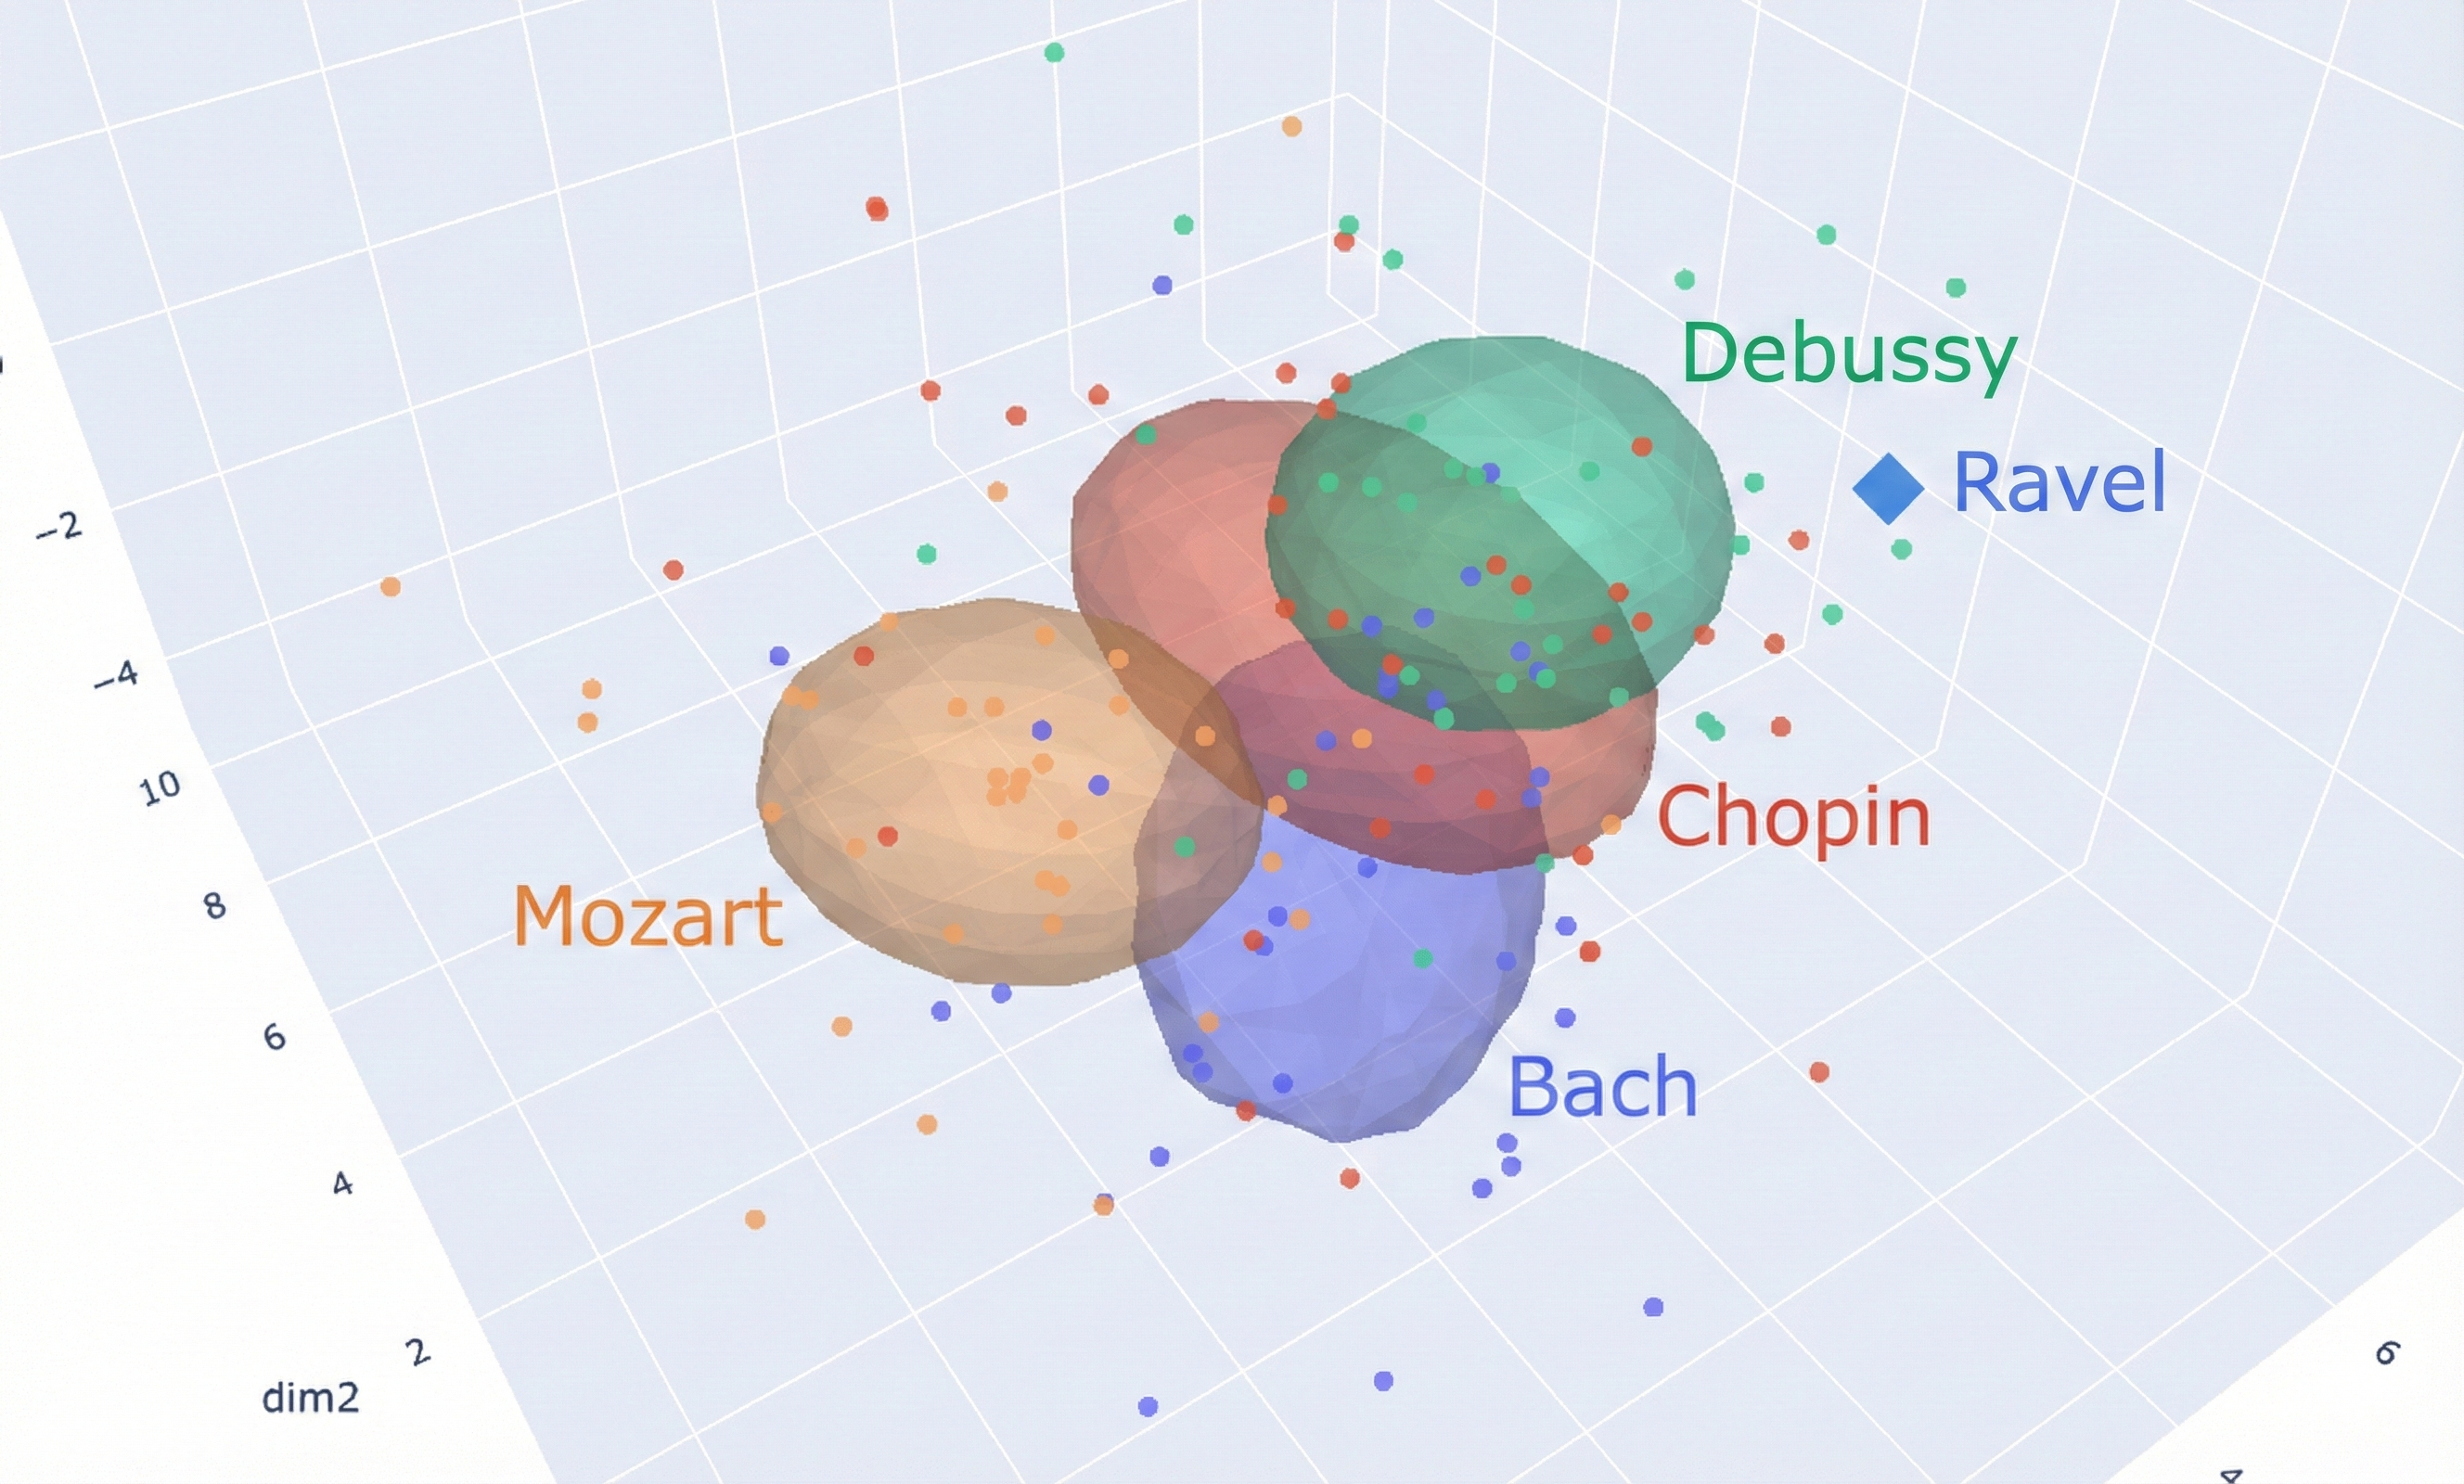
\includegraphics[width=0.85\textwidth]{ravelhighlight_cropped.png}
    }{%
        \fbox{\parbox{0.85\textwidth}{\centering (Missing figure file: ravelhighlight\_cropped.png)}}
    }
    \caption{Externer Validierungstest: Projektion von Ravels \emph{Streichquartett in F-Dur} (Diamantmarker) in die PCA-Wolken.}\label{fig:ravel}
\end{figure}

\section{Ergebnisdiskussion}
\subsection{Interpretation der Landkarte}
Die Achseninterpretation (Tabelle~\ref{tab:loadings}) ermöglicht eine musikologisch fundierte Deutung der empirischen Landkarte. Die drei Hauptkomponenten erfassen komplementäre Aspekte stilistischer Differenzierung:

\textbf{PC1 (22,3\% Varianz) -- Chromatik und Dissonanz:} Diese Achse trennt primär nach harmonischer Komplexität. Positive Ladungen auf \texttt{dissonance\_ratio}, \texttt{pitch\_class\_entropy} und \texttt{melodic\_leap\_ratio} kennzeichnen Stücke mit hoher chromatischer Dichte und Dissonanzverwendung. Die negative Korrelation mit \texttt{downbeat\_emphasis\_ratio} zeigt, dass harmonische Komplexität oft mit rhythmischer Ambiguität einhergeht.

\textbf{PC2 (16,1\% Varianz) -- Dichte versus Klarheit:} Diese Achse kontrastiert note-dichte, rhythmisch komplexe Texturen (\texttt{harmonic\_density\_mean}, \texttt{notes\_per\_beat}) gegen kadenzielle Disziplin und lange Notenwerte. Sie erfasst den Unterschied zwischen kontrapunktischer Sättigung (Bach) und galanter Klarheit (Mozart).

\textbf{PC3 (9,8\% Varianz) -- Registrale Textur:} Diese Achse misst vor allem den Tonumfang (\texttt{pitch\_range\_semitones}) und intervallische Vielfalt. Hohe Werte charakterisieren Werke, die den erweiterten Ambitus des modernen Flügels ausnutzen.

Aus dieser Interpretation ergibt sich die Cluster-Struktur:
\begin{itemize}
    \item \textbf{Bach \& Mozart} (klassische Region): Beide Komponisten liegen im PCA-Mittel auf der weniger chromatischen Seite (ähnliche PC1-Werte) im Vergleich zu Debussy -- das ist historisch plausibel und kein ``Versagen'' der Methode, sondern ein Hinweis auf gemeinsame Common-Practice-Regeln. Gleichzeitig zeigt die Trennung entlang PC2 konsistent texturale Unterschiede (kontrapunktische Dichte vs. homophone Transparenz). Im aktuellen Korpus ergibt der Tukey-Test 16 signifikante Unterschiede zwischen Bach und Mozart (davon 6 reine Zähl-/Größenmetriken wie \texttt{note\_count}, \texttt{chord\_event\_count}; ohne diese bleiben 10).
    
    \item \textbf{Debussy} (impressionistische Insel): Debussy ist auf allen drei Achsen extrempositioniert: höchste PC1-Werte (maximale Chromatik/Dissonanz), höchste PC3-Werte (extremer Ambitus) und spezifische PC2-Charakteristik. Diese dreifache Isolation quantifiziert seine revolutionäre Sonderstellung. Die 16 signifikanten Unterschiede zu Mozart (Abbildung~\ref{fig:pairwise}) untermauern, dass nahezu jede Dimension des musikalischen Raums betroffen ist.
    
    \item \textbf{Chopin} (Zwischenregion): Chopin liegt im Merkmalsraum häufig zwischen Mozart und Debussy. In den paarweisen Tukey-Tests unterscheidet sich Chopin von Debussy in 4 Merkmalen, von Mozart in 8 und von Bach in 7. Diese Asymmetrie ist konsistent mit einer intermediären Position, ist aber korpusabhängig (siehe Limitationen).
\end{itemize}

\subsection{Chopins Rolle als Brücke}
Die zweite Forschungsfrage -- "Bestätigt die quantitative Landkarte Chopins Rolle als Brückenfigur?" -- kann empirisch beantwortet werden: \textbf{Ja, mit quantifiziertem Mechanismus.}

Die musikwissenschaftliche Literatur beschreibt Chopin als Innovator, der klassische Formen beibehielt, aber harmonisch revolutionierte.\footnote{\cite{ChopinTransformations}.} Die vorliegende Datenanalyse liefert erstmals einen messbaren Beweis für diese These:

\begin{enumerate}
    \item \textbf{Visueller Befund:} In Abbildung~\ref{fig:clouds} liegt Chopin im PCA-Raum zwischen Mozart (negativere PC1-Werte) und Debussy (positivere PC1-Werte). Eine ähnliche Grobstruktur zeigt sich auch in den erzeugten 2D-Projektionen und t-SNE-Visualisierungen; dennoch bleiben Form und Abstand der Wolken abhängig von Korpuszusammensetzung und Feature-Set.
    
    \item \textbf{Statistischer Beweis:} Der Tukey-Test identifiziert die spezifischen Merkmale, die Chopin mit beiden Epochen verbinden:
    \begin{itemize}
        \item \emph{Klassische Kontinuität:} \texttt{downbeat\_emphasis\_ratio}, \texttt{std\_note\_duration}, metrische Klarheit
        \item \emph{Romantische Innovation:} \texttt{pitch\_class\_entropy} (essentielle Chromatik), \texttt{dissonance\_ratio}, \texttt{pitch\_range\_semitones}
    \end{itemize}
    
    \item \textbf{Historischer Kontext:} Die Daten stützen die These, dass Debussys Innovationen ohne Chopins Vorarbeit weniger plausibel gewesen wären. Chopin "öffnete" den stilistischen Raum: Er zeigte, dass Chromatik und Dissonanz mit klassischen Formen kompatibel sind. Debussy radikalisierte dann diese Tendenzen und löste die verbliebenen klassischen Strukturen auf.
\end{enumerate}

\subsection{Reproduzierbarkeit und Limitationen}
\textbf{Stärken der Methodik:}
\begin{itemize}
    \item Vollständige Reproduzierbarkeit durch CLI-Tools (\texttt{python3 src/aggregate\_metrics.py})
    \item Balancierte Stichprobe (n=36 pro Komponist) minimiert Verzerrungen
    \item Robuste statistische Absicherung (FDR-Korrektur, Tukey-HSD)
    \item Interpretierbare Merkmale ermöglichen musikologische Validierung
\end{itemize}

\textbf{Bekannte Limitationen:}
\begin{enumerate}
    \item \textbf{Korpus-Beschränkung:} Der Korpus ist auf Klavier-basierte Partituren aus PDMX beschränkt. Einzelne Einträge sind Sammlungen (z.\,B. ganze Zyklen) oder Duo-/Arrangements (z.\,B. \textit{Piano Duo}); diese können Verteilungen und PCA-Cluster sichtbar beeinflussen.
    \item \textbf{Normalisierung \& Stücklänge:} Zählmetriken werden in der Auswertung als Anteile oder durch Standardisierung in der PCA robust gemacht; Entropie-Maße (z.\,B. \texttt{pitch\_class\_entropy}, \texttt{rhythmic\_pattern\_entropy}) können bei sehr kurzen Stücken dennoch leicht stichprobenabhängig sein.
    \item \textbf{Erklärte Varianz:} PC1--PC3 erfassen 48,2\% der Gesamtvarianz der extrahierten Merkmale. Die verbleibenden 51,8\% liegen in höheren Dimensionen (PC4 ff.). Das bedeutet, dass stilistische Details zwar in den 36 Merkmalen modelliert sind, jedoch aufgrund der komplexen Hochdimensionalität des Datenraums in der vereinfachten 3D-Visualisierung nicht vollständig dargestellt werden können.
    \item \textbf{Symbolische Limitierung:} Die Analyse basiert auf Notentexten, nicht auf Interpretationen. Performative Aspekte (Tempo-Rubato, Pedalisierung, Agogik) bleiben unberücksichtigt.
    \item \textbf{Historische Verzerrung:} Die Korpus-Balance reflektiert nicht die tatsächliche Produktivität der Komponisten (Bach schrieb mehr Werke als im Korpus vertreten).
\end{enumerate}

Diese Limitationen sind transparent dokumentiert und bieten Ansatzpunkte für zukünftige Erweiterungen.

\subsection{Bemerkenswerte Einzelbeispiele}
Die statistischen Aggregate verbergen instruktive Extremfälle, die die Validität der Merkmalsextraktion belegen:

\textbf{Rhythmische Extreme:}
\begin{itemize}
    \item \textbf{Debussy -- La cathédrale engloutie}: Gehört im Korpus zu den Werken mit sehr hoher rhythmischer Dispersion (\texttt{std\_note\_duration}). Alternierende lange Pedalsonoritäten und kurze ornamentale Figuren erzeugen diese Varianz -- ein charakteristisches Merkmal impressionistischer Textur.
    
    \item \textbf{Bach -- Choralsammlungen}: Zeigen im Korpus teils hohe \texttt{syncopation\_ratio}-Werte durch suspensionsreiche Überbindungen. Dies dient als Plausibilitätscheck, dass die Synkopationsdetektion musikalische Substanz erfasst, nicht nur metrische Artefakte.
\end{itemize}

Diese Extremwerte wurden nach Verfeinerung der Meter-bewussten Synkopationserkennung revalidiert und bestätigen, dass die beobachteten Unterschiede genuine stilistische Signaturen sind.

\section{Fazit und Ausblick}
\subsection{Fazit}
Die zentrale Forschungsfrage -- "Kann ein kuratierter Satz interpretierbarer Merkmale eine empirische Landkarte erstellen, die stilistische Trennung und Evolution quantifiziert?" -- wurde umfassend beantwortet.

\textbf{Methodischer Erfolg:} Die entwickelte Pipeline kombiniert moderne Werkzeuge (PDMX-Archiv, \texttt{music21}, Python-Statistik) mit musikologischer Interpretierbarkeit. Im Gegensatz zu früheren Ansätzen (Lin-Jeng 1987) ermöglicht sie skalierbare, reproduzierbare Analyse bei gleichzeitiger Transparenz.

\textbf{Empirische Bestätigungen:}
\begin{enumerate}
    \item \textbf{Identifikation signifikanter Merkmale:} 29 von 36 Metriken überschreiten die FDR-Schwelle. Die stärksten Separatoren -- \texttt{pitch\_range\_semitones}, \texttt{dissonance\_ratio}, \texttt{pitch\_class\_entropy} -- erfassen zentrale Dimensionen musikhistorischer Evolution.
    
    \item \textbf{Bach/Mozart-Cluster:} Trotz stilistischer Nähe zeigt der Tukey-HSD-Test im aktuellen Korpus 16 signifikante Unterschiede zwischen Bach und Mozart (bzw. 10, wenn reine Zähl-/Größenmetriken ausgeschlossen werden). Das stützt eher die These einer teilweisen Überlappung im Merkmalsraum als eine vollständige statistische Ununterscheidbarkeit.
    
    \item \textbf{Debussy-Isolation:} 16 signifikante Unterschiede zu Mozart belegen Debussys revolutionären Sonderstatus. Die PCA positioniert ihn als isolierte "impressionistische Insel".
    
    \item \textbf{Chopins Brückenrolle:} Erstmals quantitativ belegt. Chopin bewahrt klassische kadenzielle Strukturen, während er harmonisch-melodisch in Richtung Impressionismus innoviert. Die PCA-Wolke visualisiert diese doppelte Verortung.
\end{enumerate}

Das Projekt liefert somit mehr als eine statistische Analyse: Es erstellt eine \emph{interpretierbare empirische Landkarte}, die etablierte Narrative bestätigt, präzisiert und für weitere Forschung dokumentiert.

\subsection{Ausblick}
Die entwickelte Infrastruktur bietet Ansatzpunkte für vielfältige Erweiterungen:

\textbf{Korpus-Expansion:}
\begin{itemize}
    \item \textbf{Weitere Komponisten:} Integration von Liszt, Ravel, Skrjabin, Schönberg zur Untersuchung alternativer Evolutionspfade (z.\,B.\ Romantik $\to$ Atonalität)
    \item \textbf{Andere Besetzungen:} Erweiterung auf Kammermusik, Orchesterwerke, Vokalmusik zur Validierung gattungsübergreifender Stilmerkmale
    \item \textbf{Historische Vertiefung:} Feinere zeitliche Auflösung (Früh-/Spätwerke) zur Erfassung intrakompositischer Evolution
\end{itemize}

\textbf{Methodische Erweiterungen:}
\begin{itemize}
    \item \textbf{Machine Learning:} Training interpretierbarer Klassifikatoren (Random Forest, Gradient Boosting) auf dem 30-Merkmalsraum (PCA-Eingangsmerkmale). Vergleich mit Lin-Jengs regelbasierten Ansätzen und modernen Deep-Learning-Methoden zur Bewertung von Interpretierbarkeit versus Genauigkeit. Die bereits entwickelte PCA-Basis ermöglicht direkten Übergang zu überwachtem Lernen.
    \item \textbf{Temporale Modellierung:} Integration von Markov-Modellen oder rekurrenten Netzen zur Erfassung sequenzieller Muster (z.\,B.\ charakteristische Akkordprogressionen, melodische Gesten). Die aktuelle Merkmalsmenge erfasst Statistiken über ganze Werke; sequenzielle Analysen könnten Formteile differenzieren.
    \item \textbf{Merkmals-Engineering:} Ergänzung um Dynamik-, Artikulations- und Pedal-Informationen (sofern in MusicXML kodiert). Die \texttt{music21}-Infrastruktur unterstützt diese Erweiterungen ohne Architektur-Änderungen.
    \item \textbf{Erweiterte Dissonanzklassifikation:} Differenzierung zwischen vorbereiteten/nicht vorbereiteten Dissonanzen, Erfassung von Auflösungsrichtungen (aufwärts/abwärts), Quantifizierung von Suspensions-Ketten.
\end{itemize}

\textbf{Audio-Symbolik-Brücke:}
Ein übergeordnetes Langzeitziel ist die Verbindung symbolischer Analyse (Notentext) mit audioba\-sierter Analyse (Aufnahmen). Forschungsfragen:
\begin{itemize}
    \item Manifestieren sich die identifizierten Stil-Merkmale auch in akustischen Parametern (Spektrum, Onset-Muster)?
    \item Zeigen Interpretationen historischer Aufnahmen (z.\,B.\ Cortot spielt Chopin) andere stilistische Signaturen als moderne Einspielungen?
    \item Können Audio-Klassifikatoren von der symbolischen Feature-Engineering profitieren?
\end{itemize}

\textbf{Pädagogische Anwendungen:}
Das entwickelte Annotationswerkzeug (\texttt{annotate\_musicxml.py}) könnte in musikpädagogischen Kontexten eingesetzt werden, um Schülern harmonische Analysen und Dissonanzbehandlung visuell zu vermitteln.

\section{Quellen- und Literaturverzeichnis}
\begin{thebibliography}{99}
    \bibitem{Benjamini1995} Y. Benjamini und Y. Hochberg, ``Controlling the false discovery rate: a practical and powerful approach to multiple testing,'' \emph{Journal of the Royal Stat. Society Series B}, vol. 57, no. 1, pp. 289--300, 1995.
    \bibitem{Cuthbert2010} M. S. A. Cuthbert und C. Ariza, ``music21: A Toolkit for Computer-Aided Musicology,'' in \emph{Proceedings of the 11th ISMIR}, 2010.
    \bibitem{PDMX2024} P. Long, Z. Novack, J. McAuley und T. Berg-Kirkpatrick, ``PDMX: A Large-Scale Public Domain MusicXML Dataset for Symbolic Music Processing,'' \emph{arXiv:2409.10831}, 2024.
    \bibitem{Simonetta2025} F. Simonetta, ``Style-based Composer Identification and Attribution of Symbolic Music Scores: a Systematic Survey,'' \emph{Transactions of the ISMIR}, 2025.
    \bibitem{LinJeng1987} E. F. Lin-Jeng, ``Stylistic analysis and recognition of piano sonatas of four composers -- Mozart, Chopin, Debussy, Anton Webern,'' M.S. Thesis, Rochester Institute of Technology, 1987.
    \bibitem{DebussyCharacteristics} Arabesque Conservatory, ``Claude Debussy's Musical Style: 5 Defining Characteristics,'' 2024. [Online]. Verfügbar: \url{https://www.arabesqueconservatory.com/blog/5-characteristic-traits-of-piano-music-by-debussy/}
    \bibitem{ChopinTransformations} Polish Music Center, ``Transformations of Chopin's Style,'' 2023. [Online]. Verfügbar: \url{https://polishmusic.usc.edu/research/publications/polish-music-journal/vol3no1/transformations-of-chopin/}
    \bibitem{JuFoGuide} Jugend forscht e. V., ``Leitfaden zum Verfassen der schriftlichen Arbeit,'' 2024. [Online]. Verfügbar: \url{https://www.jugend-forscht.de/fileadmin/user_upload/Downloadcenter/Teilnahme/Leitfaden_schriftliche_Arbeit.pdf}
\end{thebibliography}

\section*{Angaben zu Unterstützungsleistungen}
Die Konzeption des Projekts, die Literaturrecherche, die komplette Python-Programmierung (Korpus-Kuratierung, Parsing, Merkmalsextraktion, Statistik, Visualisierung) sowie die Auswertung und Dokumentation wurden von mir, Victor Gurbani, eigenständig erbracht. Verwendet wurden ausschließlich die in Abschnitt~7 genannten Open-Source-Bibliotheken und öffentlichen Datensätze. Mein Projektbetreuer unterstützte durch regelmäßige Feedbackgespräche zur wissenschaftlichen Methodik und zur Struktur der schriftlichen Arbeit. Es erfolgte keine finanzielle oder materielle Unterstützung durch Unternehmen oder Forschungseinrichtungen.

\newpage
\appendix
\section{Anhang: Vollständige Merkmalsdokumentation}

Dieser Anhang dokumentiert alle 36 extrahierten Merkmale der drei Säulen. Jedes Merkmal wird durch seine musikologische Bedeutung, Berechnungsmethode und Interpretation erklärt.

\subsection{Harmonische Merkmale (16)}

\subsubsection*{Akkord-Basisdaten}
\begin{description}
    \item[\texttt{chord\_event\_count}] Gesamtzahl der Akkordevents nach \texttt{chordify()}. Jedes Event repräsentiert eine simultane Sonorität über einen rhythmischen Abschnitt.
    
    \item[\texttt{chord\_quality\_total}] Anzahl der Akkorde mit klassifizierbarer Qualität (Dur/Moll/vermindert/übermäßig/andere).
\end{description}

\subsubsection*{Akkordqualitäts-Verteilung}
Alle Prozentsätze relativ zu \texttt{chord\_quality\_total}:
\begin{description}
    \item[\texttt{chord\_quality\_major\_pct}] Anteil Dur-Akkorde. Hohe Werte charakterisieren heitere, stabile Harmonik.
    
    \item[\texttt{chord\_quality\_minor\_pct}] Anteil Moll-Akkorde. Erhöhte Werte signalisieren modale Mischung oder Moll-Tonikalisierung.
    
    \item[\texttt{chord\_quality\_diminished\_pct}] Anteil verminderter Klänge. Typisch für Leitton-Akkorde (vii°) vor Kadenzen.
    
    \item[\texttt{chord\_quality\_augmented\_pct}] Anteil übermäßiger Dreiklänge. Selten; meist chromatische Durchgangsharmonien.
    
    \item[\texttt{chord\_quality\_other\_pct}] Nicht-terzenbasierte Akkorde (Quart-/Sekundschichtungen, Vorhalte, Cluster). Hohe Werte bei Debussy (z.\,B.\ \emph{Debussy: Prelude Book 2 No 12 Feux d'artifice}: 77{,}8\%).
\end{description}

\subsubsection*{Textur und Konsonanz}
\begin{description}
    \item[\texttt{harmonic\_density\_mean}] Durchschnittliche Anzahl verschiedener Tonklassen pro Akkord. Werte nahe 4 deuten auf erweiterte Harmonien hin (z.\,B.\ \emph{Chopin: Étude Op.\,10 Nr.\,11}: 3{,}785).
    
    \item[\texttt{dissonance\_ratio}] Anteil dissonanter Akkorde nach \texttt{music21.isConsonant()}. Misst vertikale Spannungsfrequenz (z.\,B.\ \emph{Debussy: Pour remercier la pluie au matin}: 0{,}845 vs.\ \emph{Mozart: Tuba Mirum}: 0{,}000).
\end{description}

\subsubsection*{Nichtakkordische Töne}
Bezogen auf die melodische Hauptstimme; Nenner ist \texttt{dissonant\_note\_count}:
\begin{description}
    \item[\texttt{dissonant\_note\_count}] Anzahl detektierter nichtakkordischer Töne.
    
    \item[\texttt{passing\_tone\_ratio}] Anteil Durchgangsnoten (schrittweise Bewegung in gleicher Richtung, Auflösung in Akkordton).
    
    \item[\texttt{appoggiatura\_ratio}] Anteil Appoggiaturen (Sprung zur Dissonanz auf betonter Zeit, schrittweise Auflösung).
    
    \item[\texttt{other\_dissonance\_ratio}] Verbleibende Dissonanzen (Wechselnoten, Antizipationen, freie Dissonanzen).
\end{description}

\subsubsection*{Römische Analyse}
\begin{description}
    \item[\texttt{roman\_chord\_count}] Erfolgreich analysierte Akkorde mit römischen Ziffern.
    
    \item[\texttt{deceptive\_cadence\_ratio}] Häufigkeit von Trugschlüssen (V--vi statt V--I).
    
    \item[\texttt{modal\_interchange\_ratio}] Anteil modaler Mischklänge (z.\,B.\ bVI in Dur aus parallelem Moll; z.\,B.\ \emph{Debussy: Petite suite}: 0{,}265).
\end{description}

\subsection{Melodische Merkmale (11)}

\subsubsection*{Registrale Merkmale}
\begin{description}
    \item[\texttt{note\_count}] Gesamtzahl melodischer Events (inkl.\ expandierter Akkordtöne). Beispiele: \emph{Bach: chorale harmonisations 241--371} 30\,349 Events; \emph{Mozart: Thema K.\,331} 55 Events.
    
    \item[\texttt{pitch\_range\_semitones}] Ambitus in Halbtönen zwischen tiefster und höchster Note. Beispiele: \emph{Mozart: Tuba Mirum} 22 Halbtöne; \emph{Debussy: Feux d'artifice} 84 Halbtöne.
\end{description}

\subsubsection*{Intervallik}
\begin{description}
    \item[\texttt{avg\_melodic\_interval}] Mittlere Intervallgröße (absolut, Halbtöne) aufeinanderfolgender Noten (z.\,B.\ \emph{Chopin: Étude Op.\,10 Nr.\,11}: 8{,}99).
    
    \item[\texttt{melodic\_interval\_std}] Standardabweichung der Intervallgrößen. Hohe Werte zeigen Wechsel zwischen Schritten und großen Sprüngen (Chopin).
    
    \item[\texttt{conjunct\_motion\_ratio}] Anteil schrittweiser Intervalle ($\leq$Ganzton).
    
    \item[\texttt{melodic\_leap\_ratio}] Anteil von Sprüngen ($>$Ganzton). Komplementär zu \texttt{conjunct\_motion\_ratio}.
\end{description}

\subsubsection*{Tonklassenverteilung}
\begin{description}
    \item[\texttt{pitch\_class\_entropy}] Shannon-Entropie der 12-Ton-Verteilung (Basis 2). Misst chromatische Dichte (z.\,B.\ \emph{Mozart: Thema K.\,331}: 2{,}296 vs.\ \emph{Chopin: 24 Préludes Op.\,28 (Gesamt)}: 3{,}566).
\end{description}

\subsubsection*{Zweistimmige Interaktion}
Sopran (oberstes System) vs.\ Bass (unterstes System):
\begin{description}
    \item[\texttt{voice\_independence\_index}] Netto-Balance zwischen Gegen- und Parallelbewegung: $(\text{contrary}  - \text{parallel}) / \text{total}$ (z.\,B.\ \emph{Chopin: Prélude Op.\,28 Nr.\,16}: $-1{,}0$; \emph{Debussy: Le petit nègre}: 0{,}667).
    
    \item[\texttt{contrary\_motion\_ratio}] Anteil gegenläufiger Bewegung.
    
    \item[\texttt{parallel\_motion\_ratio}] Anteil gleichgerichteter Bewegung.
    
    \item[\texttt{oblique\_motion\_ratio}] Anteil oblique Bewegung (eine Stimme statisch).
\end{description}

\subsection{Rhythmische Merkmale (9)}

\subsubsection*{Dauer-Statistik}
\begin{description}
    \item[\texttt{note\_event\_count}] Gesamtzahl rhythmischer Events.
    
    \item[\texttt{avg\_note\_duration}] Mittlere Notendauer (Viertelnoten-Einheiten).
    
    \item[\texttt{std\_note\_duration}] Standardabweichung der Dauern.
\end{description}

\subsubsection*{Metrische Aktivität}
\begin{description}
    \item[\texttt{notes\_per\_beat}] Durchschnittliche Events pro Schlag (z.\,B.\ \emph{Chopin: Étude Op.\,25 Nr.\,11 ``Winter Wind''}: 14{,}06 vs.\ \emph{Chopin: Nocturne n20}: 0{,}63).
    
    \item[\texttt{downbeat\_emphasis\_ratio}] Anteil starker Schläge (\texttt{beatStrength} $\geq 0{,}75$).
    
    \item[\texttt{syncopation\_ratio}] Anteil synkopischer Einträge (schwache Zeit, übergebunden über nächsten Schlag; z.\,B.\ \emph{Debussy: Nocturne}: 0{,}211; \emph{Bach: Chorale harmonisations (Compilation)}: 0{,}356).
\end{description}

\subsubsection*{Muster-Komplexität}
\begin{description}
    \item[\texttt{rhythmic\_pattern\_entropy}] Shannon-Entropie von Dauer-Trigrammen. Hohe Werte zeigen diverse rhythmische Zellen (z.\,B.\ \emph{Debussy: Nocturne}: 6{,}90 vs.\ \emph{Chopin: Étude Op.\,25 Nr.\,8}: 0{,}34).
    
    \item[\texttt{micro\_rhythmic\_density}] Anteil 4-Noten-Fenster, in denen $\geq$3 Noten schnell sind ($\leq$Sechzehntel) (z.\,B.\ \emph{Bach: Prelude BWV 1006}: 0{,}984).
\end{description}

\subsubsection*{Polyrhythmik}
\begin{description}
    \item[\texttt{cross\_rhythm\_ratio}] Anteil der Takte, in denen obere und untere Systeme verschiedene Dauernnenner verwenden (z.\,B.\ \emph{Debussy: Feuilles mortes}: 1{,}0).
\end{description}

\subsection{Zusammenfassung der Merkmals-Interpretation}

Die 36 Merkmale erfassen komplementäre Dimensionen musikalischer Gestaltung:
\begin{itemize}
    \item \textbf{Harmonik}: Erfasst vertikale Strukturen, Konsonanz/Dissonanz-Balance, nichtakkordische Verzierungen und tonale Funktionen. Debussys hohe \texttt{other\_pct} und \texttt{modal\_interchange\_ratio} quantifizieren seine harmonische Innovativität.
    
    \item \textbf{Melodik}: Misst registrale Spannweite, Intervallprofile und Stimmführungstypen. Chopins Brückenfunktion manifestiert sich in erhöhter \texttt{pitch\_class\_entropy} bei gleichzeitiger Bewahrung von \texttt{contrary\_motion\_ratio}-Werten nahe Mozart.
    
    \item \textbf{Rhythmik}: Quantifiziert metrische Organisation, synkopische Spannung und polyrhythmische Schichtung. Debussys extreme \texttt{rhythmic\_pattern\_entropy} und \texttt{cross\_rhythm\_ratio} belegen seine rhythmische Vielfalt.
\end{itemize}

Diese vollständige Dokumentation ermöglicht die Replikation und Erweiterung der Analyse auf neue Komponisten oder Repertoires.

\section{Anhang B: Reproduzierbarkeits-Leitfaden}

Dieser Anhang dokumentiert die vollständige Software-Pipeline zur exakten Replikation aller Ergebnisse. Alle Befehle und Skripte sind im Projekt-Repository verfügbar.

\subsection{Systemvoraussetzungen und Ressourcenbedarf}

\begin{itemize}
    \item \textbf{Betriebssystem}: macOS, Linux oder Windows mit WSL
    \item \textbf{Python}: Version 3.10 oder höher
    \item \textbf{Speicherplatz}: 
    \begin{itemize}
        \item PDMX-Datensatz: $\sim$56 GB (254\,077 MusicXML-Partituren)
        \item Python Virtual Environment: $\sim$600 MB
        \item Zwischenergebnisse (Features, Statistiken, Visualisierungen): $\sim$50 MB
    \end{itemize}
    \item \textbf{Rechenzeit}: 2--3 Stunden für vollständigen Durchlauf auf modernem Laptop
    \item \textbf{RAM}: Mindestens 8 GB empfohlen (16 GB für große Bach-Choralkompilationen)
\end{itemize}

\subsection{Automatisierte Installation mit Quickstart-Skript}

Das Projekt enthält ein vollautomatisches Bash-Skript, das Installation und Analyse in einem Durchlauf erledigt.

\subsubsection{Vollautomatischer Ablauf}

\begin{verbatim}
./quickstart.sh
\end{verbatim}

Das Skript führt automatisch folgende Schritte aus:
\begin{enumerate}
    \item \textbf{Abhängigkeitsprüfung}: Validiert Python-Installation und \texttt{requirements.txt}
    \item \textbf{Datensatz-Download}: Bietet interaktiven Download von Zenodo (15571083) an, falls PDMX-Verzeichnis fehlt. Unterstützt \texttt{aria2c} für parallele Downloads (16 Verbindungen) mit Fallback auf \texttt{wget}
    \item \textbf{Virtual Environment}: Erstellt isolierte Python-Umgebung im \texttt{venv/}-Verzeichnis
    \item \textbf{Dependency-Installation}: Installiert \texttt{music21}, \texttt{pandas}, \texttt{numpy}, \texttt{scipy}, \texttt{scikit-learn}, \texttt{matplotlib}, \texttt{seaborn}, \texttt{plotly}
    \item \textbf{Pipeline-Ausführung}: Führt alle 10 Analyseschritte sequenziell aus (siehe unten)
\end{enumerate}

\textbf{Alternative ohne Virtual Environment:}
\begin{verbatim}
./quickstart.sh --no-venv
\end{verbatim}
Nutzt System-Python-Installation (für conda-Nutzer oder vorinstallierte Abhängigkeiten).

\subsection{Die 10-Stufen-Analysepipeline}

Das Quickstart-Skript orchestriert folgende Schritte:

\subsubsection{Stufe 1--2: Korpus-Kuratierung und Parsing}

\textbf{[1/10] Korpus-Kuratierung}
\begin{verbatim}
python3 src/corpus_curation.py --min-rating 0
\end{verbatim}
\textit{Ausgabe}: \texttt{data/curated/solo\_piano\_corpus.csv} (144 Werke, balanciert), \texttt{solo\_piano\_mxl\_paths.txt}

\textbf{[2/10] Struktur-Parsing}
\begin{verbatim}
python3 src/score_parser.py \
    --output data/parsed/summaries.json
\end{verbatim}
\textit{Ausgabe}: JSON mit Taktzahl, Stimmenzahl, Dauern pro Partitur

\subsubsection{Stufe 3--5: Merkmals-Extraktion}

\textbf{[3/10] Harmonische Merkmale}
\begin{verbatim}
python3 src/harmonic_features.py \
    --output-csv data/features/harmonic_features.csv
\end{verbatim}
\textit{Ausgabe}: 16 harmonische Deskriptoren + Boxplots in \texttt{figures/harmonic/}

\textbf{[4/10] Melodische Merkmale}
\begin{verbatim}
python3 src/melodic_features.py \
    --output-csv data/features/melodic_features.csv
\end{verbatim}
\textit{Ausgabe}: 11 melodische Deskriptoren + Boxplots in \texttt{figures/melodic/}

\textbf{[5/10] Rhythmische Merkmale}
\begin{verbatim}
python3 src/rhythmic_features.py \
    --output-csv data/features/rhythmic_features.csv
\end{verbatim}
\textit{Ausgabe}: 9 rhythmische Deskriptoren + Boxplots in \texttt{figures/rhythmic/}

\subsubsection{Stufe 6: Dimensionsreduktion und Embedding}

\textbf{[6/10] PCA- und t-SNE-Projektionen}
\begin{verbatim}
# PCA mit 3D/2D-Visualisierung
python3 src/feature_embedding.py --method pca \
    --output figures/embeddings/pca_3d.html \
    --output-2d figures/embeddings/pca_2d.html \
    --loadings-csv data/stats/pca_loadings.csv \
    --clouds-output figures/embeddings/pca_clouds_3d.html \
    --clouds-output-2d figures/embeddings/pca_clouds_2d.html

# t-SNE mit angepassten Hyperparametern
python3 src/feature_embedding.py --method tsne \
    --perplexity 20 --tsne-composer-weight 4.0 \
    --output figures/embeddings/tsne_3d.html \
    --clouds-output figures/embeddings/tsne_clouds_3d.html
\end{verbatim}
\textit{Ausgabe}: Interaktive HTML-Scatter-Plots, Gaußsche Dichtewolken, PCA-Loadings

\subsubsection{Stufe 7--8: Statistische Signifikanz}

\textbf{[7/10] ANOVA und Tukey-HSD-Tests}
\begin{verbatim}
python3 src/significance_tests.py \
    --anova-output data/stats/anova_summary.csv \
    --tukey-output data/stats/tukey_hsd.csv
\end{verbatim}
\textit{Ausgabe}: F-Statistiken, p-Werte, Bonferroni/FDR-Flags, paarweise Vergleiche

\textbf{[8/10] Signifikanz-Visualisierungen}
\begin{verbatim}
python3 src/significance_visualizations.py --top-n 15
\end{verbatim}
\textit{Ausgabe}: Bar-Charts, Heatmaps (Paar-Counts, Mean-Difference, Sym-Log) in \texttt{figures/significance/}

\subsubsection{Stufe 9--10: Annotation und Aggregation}

\textbf{[9/10] Annotierte Referenzpartituren}
\begin{verbatim}
python3 src/generate_selected_annotations.py
\end{verbatim}
\textit{Ausgabe}: 8 farbcodierte MusicXML-Dateien (2 pro Komponist) mit Dissonanz-Labels, Akkordsymbolen und optionalen PDF-Renderings

\textbf{[10/10] Master-Aggregation}
\begin{verbatim}
python3 src/aggregate_metrics.py
\end{verbatim}
Validiert alle Outputs, druckt Korpus-Statistiken, verifiziert Konsistenz

\subsection{Manuelle Einzelschritte und Debugging}

\subsubsection{Schnelltests mit \texttt{--limit}}

Jedes Feature-Extraktions-Skript unterstützt partielle Läufe:
\begin{verbatim}
python3 src/harmonic_features.py --limit 5 \
    --output-csv /tmp/harmonic_test.csv
\end{verbatim}
Prozessiert nur die ersten 5 Partituren für Smoke-Tests.

\subsubsection{Cached Runs mit \texttt{--features-from}}

Wiederverwendung bereits berechneter Features ohne Neuberechnung:
\begin{verbatim}
python3 src/harmonic_features.py \
    --features-from data/features/harmonic_features.csv \
    --skip-plots
\end{verbatim}
Nutzt existierende CSV, erzeugt nur Statistiken (nützlich für iterative Visualisierungen).

\subsubsection{Alternative Korpus-Varianten}

Experimentiere mit unbalancierten oder entspannten Filtern:
\begin{verbatim}
python3 src/corpus_curation.py --min-rating 0 \
    --skip-license-filter \
    --max-per-composer 999 \
    --output-csv data/curated/unbalanced_corpus.csv
\end{verbatim}

\subsection{Erweiterte Funktionen}

\subsubsection{Externe Stück-Projektion}

Projiziere beliebige MusicXML-Dateien in den PCA-Raum:
\begin{verbatim}
python3 src/highlight_pca_piece.py \
    --pieces path/to/score.mxl \
    --title "Joe Hisaishi - One Summer's Day" \
    --composer "Joe Hisaishi" \
    --output highlighted_projection.html
\end{verbatim}
Unterstützt mehrere Stücke gleichzeitig mit individuellen Labels.

\subsubsection{MusicXML-Annotation mit MuseScore-Rendering}

Erzeuge farbcodierte Analysepartituren mit automatischem PDF-Export:
\begin{verbatim}
python3 src/annotate_musicxml.py \
    path/to/input.mxl \
    path/to/output_annotated.mxl \
    --renderer-template "mscore -o {output} {input}" \
    --render-format pdf
\end{verbatim}
Färbt Durchgänge (orange), Appoggiaturen (violett), andere Dissonanzen (rot), chromatische Harmonien (türkis); fügt römische Ziffern als Akkordsymbole ein.

\subsection{Validierung der Installation}

\subsubsection{Erwartete Ergebnisse}

Nach vollständigem Durchlauf sollten folgende Kennzahlen reproduziert werden:
\begin{itemize}
    \item \textbf{Korpusgröße}: Exakt 144 Partituren (36 pro Komponist)
    \item \textbf{Gesamtdauer}: 71\,585 Viertelnoten (\textasciitilde13,3 Stunden bei 90 BPM)
    \item \textbf{ANOVA-Treffer ($\alpha=0.05$)}: 29 Merkmale
    \item \textbf{FDR-robuste Merkmale ($q<0.05$)}: 29 Merkmale
    \item \textbf{PCA-Varianz (PC1--PC3)}: 48,2\% (22,3\% + 16,1\% + 9,8\%)
    \item \textbf{Tukey-Unterschiede Debussy--Mozart}: 16 signifikante Merkmale
    \item \textbf{Tukey-Unterschiede Bach--Mozart}: 10 signifikante Merkmale (bzw. 16 inklusive Zähl-/Größenmetriken)
\end{itemize}

\subsubsection{Schnelle Integritätsprüfung}

\begin{verbatim}
# Test 1: Parsing-Integrität
python3 src/score_parser.py --limit 5 \
    --output /tmp/test_parse.json
# Erwartung: 5 erfolgreiche Parses

# Test 2: Feature-Extraktion
python3 src/harmonic_features.py --limit 5 \
    --output-csv /tmp/test_harmonic.csv
# Erwartung: 5 Zeilen mit 16 Harmonie-Spalten

# Test 3: Statistik-Pipeline
python3 src/significance_tests.py --alpha 0.05
# Erwartung: anova_summary.csv mit 36 Zeilen
\end{verbatim}

\subsection{Häufige Probleme und Lösungen}

\begin{description}
    \item[\texttt{music21} Parse-Fehler bei manchen Partituren] Einige MusicXML-Dateien enthalten Formatfehler oder sind Opus-Kompilationen. \textbf{Lösung}: Alle Skripte verwenden standardmäßig \texttt{--skip-errors}, um fehlerhafte Dateien zu überspringen. Für Debugging: \texttt{--no-skip-errors} aktivieren.
    
    \item[Matplotlib Backend-Fehler auf Headless-Systemen] Server ohne Display benötigen nicht-interaktives Backend. \textbf{Lösung}: \texttt{export MPLBACKEND=Agg} vor Ausführung setzen.
    
    \item[Speicherprobleme bei Bach-Choralkompilationen] Einige Bach-Werke enthalten 100+ Choräle in einer Datei. \textbf{Lösung}: \texttt{--limit} Parameter nutzen oder RAM auf mindestens 16 GB erhöhen.
    
    \item[Abweichende PCA-Ergebnisse trotz \texttt{random\_state=42}] Unterschiedliche \texttt{scikit-learn}-Versionen können minimal andere Rotationen erzeugen. \textbf{Lösung}: Für exakte Replikation Versionen pinnen (z.\,B. via \texttt{pip freeze > requirements-lock.txt}) und die Analyse in einer frischen Umgebung ausführen.
    
    \item[Zenodo-Download schlägt fehl] API-Rate-Limits oder Netzwerkprobleme. \textbf{Lösung}: Manueller Download von \url{https://zenodo.org/records/15571083}, Extraktion nach \texttt{15571083/}.
\end{description}

\subsection{Datenformat-Spezifikationen}

\subsubsection{Korpus-CSV (\texttt{data/curated/solo\_piano\_corpus.csv})}
\begin{itemize}
    \item \texttt{composer\_label}: Normalisiert (Bach | Mozart | Chopin | Debussy)
    \item \texttt{title}: Werktitel aus PDMX-Metadaten
    \item \texttt{mxl}: Relativer Pfad zu MusicXML-Datei (z.\,B.\ \texttt{0/46/Qmaug5p...mxl})
    \item \texttt{rating}: PDMX-Qualitätsbewertung (0.0--5.0)
    \item \texttt{subset:*}: Boolsche Flags für PDMX-Subsets
\end{itemize}

\subsubsection{Feature-CSVs (\texttt{data/features/*.csv})}
Einheitliches Format für alle drei Feature-Typen:
\begin{itemize}
    \item \texttt{composer}: Komponistenname (für Gruppierung in ANOVA)
    \item \texttt{title}: Werktitel
    \item Feature-Spalten: Numerische Werte (NaN bei Extraktionsfehlern)
\end{itemize}

\subsubsection{ANOVA-Ergebnisse (\texttt{data/stats/anova\_summary.csv})}
\begin{itemize}
    \item \texttt{feature}: Merkmalsname
    \item \texttt{F\_statistic}: ANOVA-F-Wert
    \item \texttt{p\_value}: Nicht-adjustierter p-Wert
    \item \texttt{bonferroni\_sig}: Bonferroni-Signifikanz (nach $\alpha/36$)
    \item \texttt{fdr\_sig}: Benjamini-Hochberg FDR-Signifikanz ($q<0.05$)
\end{itemize}

\subsubsection{Tukey-Ergebnisse (\texttt{data/stats/tukey\_hsd.csv})}
\begin{itemize}
    \item \texttt{feature}: Merkmalsname
    \item \texttt{group1}, \texttt{group2}: Komponistenpaar
    \item \texttt{meandiff}: Mittlere Differenz
    \item \texttt{lower}, \texttt{upper}: 95\%-Konfidenzintervall
    \item \texttt{reject}: Signifikanz (True/False)
\end{itemize}

\subsection{Software-Lizenzierung und Zitierung}

\begin{itemize}
    \item \textbf{PDMX-Datensatz}: Public Domain, verfügbar unter \url{https://zenodo.org/records/15571083}. Zitierung: \cite{PDMX2024}
    \item \textbf{Analysecode}: Siehe \texttt{LICENSE}-Datei im Repository
    \item \textbf{Extrahierte Features}: Abgeleitete Daten, frei verwendbar für akademische Zwecke unter Nennung dieser Arbeit
    \item \textbf{Dependencies}: Alle verwendeten Bibliotheken (\texttt{music21}, \texttt{scikit-learn}, etc.) sind Open Source (BSD/MIT-Lizenzen)
\end{itemize}

Dieser Leitfaden ermöglicht vollständige Reproduktion aller Ergebnisse sowie deren Erweiterung auf neue Fragestellungen. Bei Problemen: GitHub-Issues im Repository oder Kontakt über die im Hauptdokument angegebene Adresse.

\end{document}